\documentclass[12pt]{article}
\usepackage{ctex}
\usepackage{amsmath,amsthm}
\usepackage{graphicx,float}
\usepackage{fancyhdr}
\usepackage{array}
\usepackage[a4paper, total={7in,9in}]{geometry}

\graphicspath{{../image/}}

\renewcommand{\arraystretch}{1.8}

\fancyhf{}
\fancyhf[HL]{Pre S.4 Summer course}
\fancyhf[FR]{P.\thepage}

\newtheorem*{theorem}{Theorem}
\newtheorem{example}{示例}

\begin{document}
    \pagestyle{fancy}
    \begin{center}
        \textbf{Factorization}
    \end{center}

    回顧因數分解概念,根據我們在小學學到的知識,某個數字(如18)的因數可用下列方式表示: \begin{align*}
        18&=1\times 18\\
        &=2\times 9\\
        &=3\times 6
    \end{align*}
    因此,在這個例子中,我們有 $1,2,3,6,9,18$ 作為 $18$ 的因子。同樣地,當我們進入多項式的討論時,因數分解的概念仍然有效,但因式分解的運算會變得不清楚,而需要對多項式本質有更多理解。

    觀察下列算式,已知 \begin{align*}
        x\cdot x=x^2
    \end{align*} 因此\begin{align*}
        x^2-2x&=x(x-2)\\
        x^3+4x^2&=x^2(x+4)
    \end{align*}

    若認為上面的表達式有點含糊,回憶分配律:\begin{align*}
        a(b+c)&=ab+ac\\
        (a+b)c&=ac+ab
    \end{align*} 並將倒推表達式。注意:因式分解只是展開數式的反向操作。\begin{align*}
        x(x-2)&=x\cdot x-x\cdot 2\\
        &=x^2-2x\\
        x^2(x+4)&=x^2\cdot x+x^2\cdot 4\\
        &=x^3+4x^2
    \end{align*}

    由於 $x^2\cdot x$ 可被視爲 $x\cdot x\cdot x$, 因此 3 個 $x$ 相乘可得 $x^3$.

    然而,並非每個多項式都像我們所看到的那樣簡單。對於物理學中存在的一些表達式,我們會遇到類似這樣的情況:\begin{align*}
        x^2+3x+4&=0
    \end{align*}

    我們有不同的方法以求$x$的值。接下來將使用之前學過的恆等式。

    讓我們先溫習一下我們對因式分解的理解。
    \subsection*{Exercise}
    \begin{enumerate}
        \item 例出下列數字的所有因子,包括負數:\begin{align*}
            &a)\ 4&&b)\ 6&&c)\ 12&&d)\ 15\\
            &e)\ 32&&f)\ 44&&g)\ 52&&h)\ 80
        \end{align*}
        \item 對下列各項進行質因數分解:\begin{align*}
            &a)\ 4&&b)\ 6&&c)\ 12&&d)\ 15\\
            &e)\ 32&&f)\ 44&&g)\ 52&&h)\ 80
        \end{align*}
        \item 因式分解:\begin{align*}
            &a)\ x^2+x&&b)\ x-xy&&c)\ x^4+2x^2+2x&&d)\ x^3-2x
        \end{align*}
    \end{enumerate}

    \begin{center}
        \textbf{以恆等式進行因式分解}
    \end{center}

    回顧以下展開式:\begin{align*}
        (x+y)^2&=x^2+2xy+y^2\\
        (x-y)^2&=x^2-2xy+y^2\\
        (x+y)(x-y)&=x^2-y^2
    \end{align*}

    我們應該注意到,等號是雙向有意義的,也就是說,每當左手邊等於右手邊,右手邊就立即等於左手邊。因此,我們可能會從相反的方向來看上面的情況。\begin{align*}
        x^2+2xy+y^2&=(x+y)^2\\
        x^2-2xy+y^2&=(x-y)^2\\
        x^2-y^2&=(x+y)(x-y)
    \end{align*}

    這稱為\textbf{恆等式因式分解}。

    \begin{example}
        因式分解 $x^2+2x+1$.
    \end{example}
    \textit{ Sol. }\begin{align*}
        x^2+2x+1&=(x)^2+2(x)(1)+(1)^2\\
        &=(x+1)^2
    \end{align*}

    \begin{example}
        因式分解 $x^2+4x+4$.
    \end{example}
    \textit{ Sol. }\begin{align*}
        x^2+4x+4&=(x)^2+2(x)(2)+(2)^2\\
        &=(x+2)^2
    \end{align*}

    \begin{example}
        因式分解 $x^2-2x+1$.
    \end{example}
    \textit{ Sol. }\begin{align*}
        x^2-2x+1&=(x)^2-2(x)(1)+(1)^2\\
        &=(x-1)^2
    \end{align*}

    \begin{example}
        因式分解 $x^2-4x+4$.
    \end{example}
    \textit{ Sol. }\begin{align*}
        x^2-4x+4&=(x)^2-2(x)(2)+(2)^2\\
        &=(x-2)^2
    \end{align*}

    \begin{example}
        因式分解 $x^2-1$.
    \end{example}
    \textit{ Sol. }\begin{align*}
        x^2-1&=(x)^2-(1)^2\\
        &=(x+1)(x-1)
    \end{align*}

    \begin{example}
        因式分解 $x^2-9$.
    \end{example}
    \textit{ Sol. }\begin{align*}
        x^2-9&=(x)^2-(3)^2\\
        &=(x+3)(x-3)
    \end{align*}

    讓我們運用恆等式做些簡單的因式分解練習。

    \subsection*{Exercise}
    \begin{enumerate}
        \item 因式分解:\begin{align*}
            &a)\ x^2+6x+9&&b)\ x^2+8x+16&&c)\ x^2+10x+25&&d)\ x^2+16x+64\\
            &e)\ 2x^2+12x+18&&f)\ 4x^2+32x+64&&g)\ 6x^2+60x+150&&h)\ 8x^2+128x+512\\
            &i)\ x^3+6x^2+9x&&j)\ x^5+8x^4+16x^3&&k)\ x^8+10x^6+25x^4&&l)\ x^9+16x^5+64x\\
        \end{align*}
        \item 因式分解:\begin{align*}
            &a)\ x^2-6x+9&&b)\ x^2-8x+16&&c)\ x^2-10x+25&&d)\ x^2-16x+64\\
            &e)\ 2x^2-12x+18&&f)\ 4x^2-32x+64&&g)\ 6x^2-60x+150&&h)\ 8x^2-128x+512\\
            &i)\ x^3-6x^2+9x&&j)\ x^5-8x^4+16x^3&&k)\ x^8-10x^6+25x^4&&l)\ x^9-16x^5+64x\\
        \end{align*}
        \item 因式分解:\begin{align*}
            &a)\ x^2-9&&b)\ x^2-16&&c)\ x^2-25&&d)\ x^2-64\\
            &e)\ 2x^2-18&&f)\ 4x^2-64&&g)\ 6x^2-150&&h)\ 8x^2-512\\
            &i)\ x^3-9x&&j)\ x^5-16x^3&&k)\ x^8-25x^4&&l)\ x^9-64x\\
        \end{align*}
        \item 因式分解:\begin{align*}
            &a)\ x^2+2ax+a^2&&b)\ x^2+8x+16-b^2\\
            &c)\ x^2+10x+25-y^2+2yc-c^2&&d)\ ax^2+16a^2x+64a^3\\
            &e)\ 2x^2+12xy+18y^2&&f)\ 4(x+y)^2+32(x^2-y^2)+64(x-y)^2
        \end{align*}
    \end{enumerate}

    \begin{center}
        \textbf{以更多恆等式進行因式分解}
    \end{center}

    為提高對因式分解的認知,我們將學習更多恆等式式以更熟練地運用它們。

    我們已有二次多項式,所以我們可以進階到三次多項式\begin{align*}
        (x+y)^3&=x^3+3x^2y+3xy^2+y^3\\
        (x-y)^3&=x^3-3x^2y+3xy^2-y^3\\
        (x+y)(x^2-xy+y^2)&=x^3+y^3\\
        (x-y)(x^2+xy+y^2)&=x^3-y^3
    \end{align*}

    為清晰起見,我們將為其提供一個證明。\begin{enumerate}
        \item 對於 $(x+y)^3=x^3+3x^2y+3xy^2+y^3$:\begin{align*}
            (x+y)^3&=(x+y)(x+y)^2\\
            &=(x+y)(x^2+2xy+y^2)\\
            &=x^3+3x^2y+3xy^2+y^3
        \end{align*}
        \item 對於 $(x-y)^3=x^3-3x^2y+3xy^2-y^3$:\begin{align*}
            (x-y)^3&=(x-y)(x-y)^2\\
            &=(x-y)(x^2-2xy+y^2)\\
            &=x^3-3x^2y+3xy^2-y^3
        \end{align*}
        \item 對於 $(x+y)(x^2-xy+y^2)=x^3+y^3$:\begin{align*}
            (x+y)(x^2-xy+y^2)&=x^3+x^2y-x^2y-xy^2+xy^2+y^3\\
            &=x^3+y^3
        \end{align*}
        \item 對於 $(x-y)(x^2+xy+y^2)=x^3-y^3$:\begin{align*}
            (x-y)(x^2+xy+y^2)&=x^3-x^2y+x^2y-xy^2+xy^2-y^3\\
            &=x^3-y^3
        \end{align*}
    \end{enumerate}
    
    讓我們通過一些例子來提升我們對其原理的熟練度。

    \begin{example}
        因式分解 $x^3+3x^2+3x+1$.
    \end{example}
    \textit{ Sol. }\begin{align*}
        x^3+3x^2+3x+1&=(x)^3+3(x)^2(1)+3(x)(1)^2+(1)^3\\
        &=(x+1)^3
    \end{align*}

    \begin{example}
        因式分解 $x^3+6x^2+12x+8$.
    \end{example}
    \textit{ Sol. }\begin{align*}
        x^3+6x^2+12x+8&=(x)^3+3(x)^2(2)+3(x)(2)^2+(2)^3\\
        &=(x+2)^3
    \end{align*}

    \begin{example}
        因式分解 $x^3-3x^2+3x-1$.
    \end{example}
    \textit{ Sol. }\begin{align*}
        x^3-3x^2+3x-1&=(x)^3-3(x)^2(1)+3(x)(1)^2-(1)^3\\
        &=(x-1)^3
    \end{align*}

    \begin{example}
        因式分解 $x^3-6x^2+12x-8$.
    \end{example}
    \textit{ Sol. }\begin{align*}
        x^3-6x^2+12x-8&=(x)^3-3(x)^2(2)+3(x)(2)^2-(2)^3\\
        &=(x-2)^3
    \end{align*}

    \begin{example}
        因式分解 $x^3+1$.
    \end{example}
    \textit{ Sol. }\begin{align*}
        x^3+1&=(x)^3+(1)^3\\
        &=(x+1)(x^2-x+1)
    \end{align*}

    \begin{example}
        因式分解 $x^3+8$.
    \end{example}
    \textit{ Sol. }\begin{align*}
        x^3+8&=(x)^3+(2)^3\\
        &=(x+2)(x^2-2x+4)
    \end{align*}

    \begin{example}
        因式分解 $x^3-1$.
    \end{example}
    \textit{ Sol. }\begin{align*}
        x^3-1&=(x)^3-(1)^3\\
        &=(x-1)(x^2+x+1)
    \end{align*}

    \begin{example}
        因式分解 $x^3-8$.
    \end{example}
    \textit{ Sol. }\begin{align*}
        x^3-8&=(x)^3-(2)^3\\
        &=(x-2)(x^2+2x+4)
    \end{align*}

    現在我們對3次多項式因式分解有了認識,讓我們做些基本的恆等式練習。

    \subsection*{Exercise}
    \begin{enumerate}
        \item 因式分解:\begin{align*}
            &a)\ x^3+9x^2+27x+27&&b)\ x^3+12x^2+48x+64&&c)\ x^3+15x^2+75x+125\\
            &d)\ 2x^3+18x^2+54x+54&&e)\ 3x^3+36x^2+144x+192&&f)\ 5x^3+75x^2+375x+625\\
        \end{align*}
        \item 因式分解:\begin{align*}
            &a)\ x^3-9x^2+27x-27&&b)\ x^3-12x^2+48x-64&&c)\ x^3-15x^2+75x-125\\
            &d)\ 2x^3-18x^2+54x-54&&e)\ 3x^3-36x^2+144x-192&&f)\ 5x^3-75x^2+375x-625\\
        \end{align*}
        \item 因式分解:\begin{align*}
            &a)\ x^3+27&&b)\ x^3+12x^2+48x+64&&c)\ x^3+125\\
            &d)\ 2x^3+54&&e)\ 3x^3+192&&f)\ 5x^3+625\\
        \end{align*}
        \item 因式分解:\begin{align*}
            &a)\ x^3-27&&b)\ x^3-64&&c)\ x^3-125\\
            &d)\ 2x^3-54&&e)\ 3x^3-192&&f)\ 5x^3-625\\
        \end{align*}
    \end{enumerate}

    \begin{center}
        \textbf{以十字相乘法進行因式分解}
    \end{center}

    從現在開始,我們將深入探究一個重要問題:如何解以下形式: $$x^2+px+q$$ 或為更廣汎的形式 $$ax^2+bx+c$$ 的二次方程? 假設 $x^2+px+q$ 可被分解爲 $$(x+a)(x+b)$$ 就相當於說 $$(x+a)(x+b)=x^2+px+q$$ 也就是説 $$x+(a+b)x+ab=x^2+px+q$$

    比較同類項,可見 \begin{align*}
        \begin{cases}
            a+b=p\\
            ab=q
        \end{cases}
    \end{align*}

    這給了我們一個提示,我們應先分解常數 $q$ 再利用$a+b=p$求得 $a,b$ 的正確值。

    總結步驟:\begin{enumerate}
        \item 通過比較同類項,求 $p,q$ 的值。
        \item 嘗試寫出q的每對因子。
        \item 檢查每對因子的和。 如符合 $a+b=p$,則為正確答案。
        \item 寫下 $(x+a)(x+b)$。
    \end{enumerate}

    \begin{example}
        因式分解 $x^2+4x+3$.
    \end{example}

    \textit{ Sol.}1:求 $p$ 和$q$.
    \begin{align*}
        p=4, q=3
    \end{align*}
    \indent \indent 2:分解 $q$ (包含負數因子對).
    \begin{align*}
        3&=1\cdot 3\\
        &=(-1)\cdot(-3)
    \end{align*}
    \indent \indent 3:檢查 $a+b=p$ (包括負數因子對).
    \begin{align*}
        1+3&=4\\
        (-1)+(-3)&=-4
    \end{align*}
    \indent \indent \indent 由於 $p=4$,所以 $a=1,b=3$為正確答案\\
    \indent \indent 4:總結。
    \begin{align*}
        x^2+4x+3=(x+1)(x+3)
    \end{align*}

    我們應確保因式分解後的表達式可以展開為原本的多項式。\begin{align*}
        (x+1)(x+3)&=x(x+3)+(x+3)\\
        &=x^2+3x+x+3\\
        &=x^2+4x+3
    \end{align*}

    這說明我們的步驟正確。有數學家認為上述步驟可以有更緊凑的表示方式。這個方法我們將其稱為\textbf{十字相乘法}。
    
    \begin{example}
        利用十字相乘法因式分解 $x^2+4x+3$。
    \end{example}

    \textit{ Sol.}由於 $3=1\cdot 3=(-1)\cdot(-3)$,
    \begin{figure}[H]
        \centering
        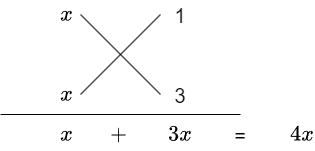
\includegraphics[scale=0.6]{cross-method}
    \end{figure}
    \indent \indent 即 $x^2+4x+3=(x+1)(x+3)$。

    我們可以通過以下練習來熟習十字相乘法的運用。

    \subsection*{Exercise}
    \begin{enumerate}
        \item 以十字相乘法因式分解:\begin{align*}
            &a)\ x^2+6x+8&&b)\ x^2+9x+18&&c)\ x^2+7x+6\\
            &d)\ x^2-6x+8&&e)\ x^2-9x+18&&f)\ x^2-7x+6\\
            &g)\ x^2+6x-27&&h)\ x^2+9x-22&&i)\ x^2+7x-30\\
            &j)\ x^2-6x-27&&k)\ x^2-9x-22&&l)\ x^2-7x-30
        \end{align*}
        \item 以十字相乘法因式分解:\begin{align*}
            &a)\ 2x^2+12x+16&&b)\ 3x^2+27x+54&&c)\ 5x^2+35x+30\\
            &d)\ 7x^2-42x+56&&e)\ -11x^2+99x-198&&f)\ -3x^2+21x-18
        \end{align*}
    \end{enumerate}

    \begin{center}
        \textbf{Solving quadratic equations by factor method}
    \end{center}

    為解二次方程,我們得知以下幾點\begin{theorem}
        若 $ab=0$, 則 $a=0$ 或 $b=0$。
    \end{theorem}

    從以上可見,若 $(x-\alpha)(x-\beta)=0$,則 $x-\alpha=0$ 或 $x-\beta=0$。因此方程的 \textbf{解} 為 $x=\alpha$ 或 $x=\beta$.

    \begin{example}
        解 $x^2-4x+3=0$.
    \end{example}

    \textit{ Sol. }通過因式分解,可得 $(x-1)(x-3)=0$,因此 $x=1$ 或 $x=3$ 為方程的解。

    \begin{example}
        解 $x^2+4x+3=0$.
    \end{example}

    \textit{ Sol. }通過因式分解,可得 $(x+1)(x+3)=0$,因此 $x=-1$ 或 $x=-3$ 為方程的解。

    當我遇到方程有兩個根,而兩個根是重複的話,我們只需列明其中一個根即可。

    \begin{example}
        解 $x^2+4x+4=0$.
    \end{example}

    \textit{ Sol. }通過因式分解,可得 $(x+2)^2=0$,則 $x=-2$ 是唯一解

    \subsection*{Exercise}
    \begin{enumerate}
        \item 解方程:\begin{align*}
            &a)\ 2x^2+12x+16=0&&b)\ 3x^2+27x+54=0&&c)\ 5x^2+35x+30=0\\
            &d)\ 7x^2-42x+56=0&&e)\ -11x^2+99x-198=0&&f)\ -3x^2+21x-18=0
        \end{align*}
        \item 解方程:\begin{align*}
            &a)\ x^2+6x+9=0&&b)\ x^2+8x+16=0&&c)\ x^2+10x+25=0\\
            &d)\ x^2+16x+64=0&&e)\ 2x^2-12x+18=0&&f)\ 4x^2-32x+64=0\\
            &g)\ 6x^2-60x+150=0&&h)\ 8x^2-128x+512=0&&i)\ x^3-9x=0\\
            &j)\ x^5-16x^3=0&&k)\ x^8-25x^4=0&&l)\ x^9-64x=0
        \end{align*}
    \end{enumerate}

    \begin{center}
        \textbf{使用公式求解二次方程}
    \end{center}

    應注意,並不是所有二次多項式都可以完美分解。例如以下等式:$$x^2+6x-6=0$$

    我們可以見到對於左側,如果$x=0$, 則表達式計算結果大於 $0$; 若 $x=1$, 則表達式計算結果小於 $0$由此可想象存在$0<x<1$使等式成立。
    
    至於準確解,我們引入根號 $\sqrt{k}$ 以解 $x^2=k$. 需要重要記得的一點是,正數和負數在平方后都等於正數。即 $(\sqrt{x})^2=x$ 及 $(-\sqrt{x})^2=x$ 當 $x>0$.

    至於一般式 $ax^2+bx+c=0$,其解可以用以下形式表達:$$\frac{-b\pm\sqrt{b^2-4ac}}{2a}$$其中加減號$\pm$同時表示一正一減兩個解。這代表只要$x$可滿足此二次方程,則: $$x=\frac{-b+\sqrt{b^2-4ac}}{2a}\textrm{ 或 }x=\frac{-b-\sqrt{b^2-4ac}}{2a}$$ 
    
    此表達方式來自配分法,其過程較爲複雜。為證明其真確性,我們將以抽象的方式的寫法展示過程,而確實證明可參閲稍後的二次多項式圖表部分。

    此為二次方程的證明:\begin{align*}
        ax^2+bx+c&=0\\
        a(x^2+\frac{b}{a}x)+c&=0\\
        a(x^2+2\frac{b}{2a}x+\frac{b^2}{4a^2}-\frac{b^2}{4a^2})+c&=0\\
        a(x+\frac{b}{2a})^2&=\frac{b^2-4ac}{4a}\\
        (x+\frac{b}{2a})^2&=\frac{b^2-4ac}{4a^2}\\
        x+\frac{b}{2a}&=\pm\frac{\sqrt{b^2-4ac}}{2a}\\
        x&=\frac{-b\pm\sqrt{b^2-4ac}}{2a}
    \end{align*}

    以 下 為 一 些 二 次 方 程 的 應 用:

    \begin{example}
        解$x^2+7x-9=0$。
    \end{example}

    \textit{ Sol.} $a=1$, $b=7$, $c=-9$ \begin{align*}
        x&=\frac{-b\pm\sqrt{b^2-4ac}}{2a}\\
        &=\frac{-7\pm\sqrt{7^2-4\cdot 1\cdot (-9)}}{2}\\
        &=\frac{-7\pm\sqrt{85}}{2}
    \end{align*}

    \begin{example}
        解 $2x^2+3x-4=0$ 。
    \end{example}

    \textit{ Sol.}  $a=2$, $b=3$, $c=-4$ \begin{align*}
        x&=\frac{-b\pm\sqrt{b^2-4ac}}{2a}\\
        &=\frac{-3\pm\sqrt{3^2-4\cdot 2\cdot (-4)}}{4}\\
        &=\frac{-3\pm\sqrt{41}}{4}
    \end{align*}

    現 在 可 以 嘗 試 使 用 二 次 方 程 公 式 求 解 任 何 二 次 方 程 。

    \subsection*{Exercise}

    \begin{enumerate}
        \item 求解以下二次方程:\begin{align*}
            &a)\ 3x^2-12x-26=0&&b)\ 7x^2-27x+54=0&&c)\ 4x^2+35x+1=0\\
            &d)\ 2x^2-33x+6=0&&e)\ -11x^2+89x-18=0&&f)\ -3x^2+21x-18=0
        \end{align*}
        \item 求解以下二次方程,並以$k$表示答案:\begin{align*}
            &a)\ 3kx^2-x-2=0&&b)\ 7x^2-27x+k=0&&c)\ kx^2+35x+1=0\\
            &d)\ 2x^2-3kx+6=0&&e)\ -11x^2+kx-k=0&&f)\ -kx^2+21x-k^2=0
        \end{align*}
    \end{enumerate}

    \begin{center}
        \textbf{實根的存在性}
    \end{center}

    留意在二次方程公式中 $$\frac{-b\pm \sqrt{b^2-4ac}}{2a}$$ 開方部分 $b^2-4ac$對根的性質有很大的影響,我們稱其爲 \textbf{判別式}代表其可判斷根的特性。若此部分 $\geq 0$則公式有實數答案;若此部分 $< 0$, 則公式沒有實數答案。 在以前,它殺死了很多數學家,但從現在開始,讓我們為它定義一
    個新的概念。

    我們將定義一個新元素$i$, 使其滿足方程: $$i^2=-1$$ 並對於所有正數 $k$可寫 $\sqrt{-k}=i\sqrt{k}$。我們稱 $i$ 為虛數,因爲它不是實數。

    從這個意義上說,當 $b^2-4ac<0$, 我 們 可 以 用 一 個 更 合 適 的 書 寫 形 式 ,即 $x+yi$, 使得每個解都可以完整表達。我們將這種形式的數字稱為\textbf{複數}, 其中$x, y$是實數。

    從這裡開始,讓我們用表格寫下根的性質的結論:

    \begin{center}
        \begin{tabular}{|c|c|c|}
            \hline
            $\Delta=b^2-4ac$&根&性質\\
            \hline
            $>0$&$\dfrac{-b\pm\sqrt{\Delta}}{2a}$&相異實根\\
            \hline
            $=0$&$\dfrac{-b}{2a}$&重根\\
            \hline
            $<0$&$\dfrac{-b\pm\sqrt{-\Delta}i}{2a}$&沒有實根 (2 虛數根)\\
            \hline
        \end{tabular}
    \end{center}

    由此,我們現在可以在計算根值之前確定根的性質。
    \begin{example}
        辨別下列根的性質。如果它有實根,則求解。\begin{enumerate}
            \item[(a)] $7x^2+5x-10=0$.
            \item[(b)] $81x^2-18x+1=0$.
            \item[(c)] $20x^2+19x+10=0$.
        \end{enumerate}
    \end{example}

    \textit{ Sol.}\begin{enumerate}
        \item[(a)] 檢 查 判 別 式 $\Delta=b^2-4ac=5^2-4(7)(-10)=305>0$, , 因 此 它 有 2 個 不 同 的 實 根 。 代 $\Delta$, \begin{align*}
            x=\frac{-b\pm\sqrt{\Delta}}{2a}=\frac{-5\pm\sqrt{305}}{14}
        \end{align*}
        \item[(b)] 檢 查 判 別 式 $\Delta=b^2-4ac=(-18)^2-4(81)(1)=0$, 因 此 它 有 1 個 實 根 。 代 $\Delta$\begin{align*}
            x=\frac{-b}{2a}=\frac{18}{162}=\frac{1}{9}
        \end{align*}
        \item[(c)] 檢 查 判 別 式 $\Delta=b^2-4ac=19^2-4(20)(10)=-439<0$, 因 此 它 沒 有 實 根 。
    \end{enumerate}

    同時注意,如果我們知道一些未知二次方程的根的性質,我們可以根據判別式的命題來計算未知數。

    \begin{example}
        已知二次方程 $kx^2-4x+k=0$ 只有一個實數根,$k$為實數 。解方程。
    \end{example}

    \textit{ Sol.}通過檢查判別式,我們得到以下結果:\begin{align*}
        (-4)^2-4\cdot k\cdot k&=0\\
        k&=\pm 2
    \end{align*}
    \indent \indent 因此方程應該是 $2x^2-4x+2=0$ 或 $-2x^2-4x-2=0$,分別有 $x=2$ 及 $x=-2$ 作爲根。

    \subsection*{Exercise}
    \begin{enumerate}
        \item 判斷下 列 二 次 方 程 根 的 性 質 :\begin{align*}
            &a)\ -390x^2-988x+794=0&&b)\ 82x^2+290x+759=0&&c)\ -924x^2-708x+959=0\\
            &d)\ -265x^2+336x-685=0&&e)\ 845x^2+396x-501=0&&f)\ -246x^2+16x-318=0
        \end{align*}
        \item 如 果 下 列 二 次 方 程 都 只 有 一 個 實 數 根 , 求 $k$ 的 值 。\begin{align*}
            &a)\ kx^2-2x+9=0&&b)\ 82x^2+kx+79=0&&c)\ -24x^2-70x+4k=0\\
            &d)\ -kx^2+36x-k=0&&e)\ 8kx^2+3kx-51=0&&f)\ 2kx^2+(3k-6)x-4k-8=0
        \end{align*}
    \end{enumerate}

    \begin{center}
        \textbf{韋達定理:根和係數之間的關係}
    \end{center}

    我們現在可以進一步深入探討比較抽象的内容,在上一部分中,我們發現判別式可告訴我們二次方程根的性質,當我們看到根以重數計算,根的數量始終等於2。這並不奇怪,因為我們總是可以想到將兩次方程分解為兩個線性因式的乘積,因此我們可以假設始終有2個根。

    現在我們要研究根和係數之間的關係,因此我們有一個由數學家創建的新遊戲,稱為代數。假設我們有一個形式為_的二次方程,並且該方程有根$\alpha$和$\beta$,這可能不是實數,但我們仍然可以用複數表示它們。如果我們將這些詞翻譯成數學表示: $$(x-\alpha)(x-\beta)=0=x^2-px+q$$ It is clear that the left-hand side is exactly equal to the right-hand side. We then expand the left-hand side to the following form: $$x^2-(\alpha+\beta)x+\alpha\beta=x^2+px+q$$ This takes us to the relation between roots and coefficients by comparing like terms $$\begin{cases}
        \alpha+\beta=-p\\ 
        \alpha\beta=q
    \end{cases}$$

    The simultaneous equations above is a system of relation called the \textbf{Vieta's formula}, which has another name called the \textbf{sum of roots} for the first equation and \textbf{product of roots} for the second equation.

    In order to generalize the relationship further to any quadratic equations in the form of $ax^2+bx+c=0$ with real numbers $a,b,c$, we take the following transformation $$ax^2+bx+c=0 \implies x^2+\frac{b}{a}x+\frac{c}{a}=0$$ so that the equation is identical to what we have investigated just a moment before by taking $p=\frac{b}{a}$ and $q=\frac{c}{a}$. Therefore, the general Vieta's formula becomes $$\begin{cases}
        \alpha+\beta=-\frac{b}{a}\\ 
        \alpha\beta=\frac{c}{a}
    \end{cases}$$

    \begin{example}
        Find the sum of roots and product of roots for the quadratic equation $3x^2+2x+9=0$.
    \end{example}

    \textit{ Sol.}By letting $\alpha$ and $\beta$ to be the roots of the equation, using Vieta's formula we get $$\begin{cases}
        \alpha+\beta=-\frac{2}{3}\\ 
        \alpha\beta=\frac{9}{3}=3
    \end{cases}$$

    \begin{example}
        Construct a quadratic equation with integral coefficients using $\frac{1}{2}$ and $\frac{2}{3}$ as roots.
    \end{example}

    \textit{ Sol.}Using Vieta's formula we get $$\begin{cases}
        \alpha+\beta=\frac{1}{2}+\frac{2}{3}=\frac{5}{6}\\ 
        \alpha\beta=\frac{1}{2}\cdot \frac{2}{3}=\frac{1}{3}
    \end{cases}$$
    \indent \indent Hence, the quadratic equation we need is given by $$x^2-(\alpha+\beta)x+\alpha\beta=0 \implies x^2-\frac{5}{6}x+\frac{1}{3}=0 \implies 6x^2-5x+2=0$$

    \subsection*{Exercise}
    \begin{enumerate}
        \item Find the sum of roots and product of roots for the following quadratic equations:\begin{align*}
            &a)\ -390x^2-988x+794=0&&b)\ 82x^2+290x+759=0&&c)\ -924x^2-708x+959=0\\
            &d)\ -265x^2+336x-685=0&&e)\ 845x^2+396x-501=0&&f)\ -246x^2+16x-318=0\\
            &g)\ kx^2-2x+9=0&&h)\ 82x^2+kx+79=0&&i)\ -24x^2-70x+4k=0\\
            &j)\ -kx^2+36x-k=0&&k)\ 8kx^2+3kx-51=0&&l)\ 2kx^2+(3k-6)x-4k-8=0
        \end{align*}
        \item Construct, for each pair of roots stated below, a quadratic equation with integral coefficients respectively.\begin{enumerate}
            \item $\frac{2}{5}$ and $-\frac{6}{7}$.
            \item $\frac{3}{2}$ and $\frac{7}{4}$.
            \item $4$ and $-4$.
            \item $5$ and $-\frac{2}{7}$.
        \end{enumerate}
    \end{enumerate}

    \begin{center}
        \textbf{More about roots of equations (Optional)}
    \end{center}

    To construct a quadratic equation, we shall first figure out the roots of the required polynomial. Most of the times we are not going to be given roots, but we will need to compute from other given information.

    \begin{example}
        It is given that $\alpha$ and $\beta$ are roots of the quadratic polynomial $ax^2+bx+c$. Construct a quadratic polynomial with roots $\alpha^2$ and $\beta^2$ in terms of $a,b,c$.
    \end{example}

    \textit{ Sol.} To construct the required polynomial we shall find by Vieta's formula the value of $\alpha^2+\beta^2$ and $\alpha^2\beta^2$. It is known that from our assumption that \begin{align*}
        \begin{cases}
            \alpha+\beta=-\frac{b}{a}\\
            \alpha\beta=\frac{c}{a}
        \end{cases}
    \end{align*}
    Therefore, the required sum of roots and product of roots are \begin{align*}
        \alpha^2+\beta^2&=(\alpha+\beta)^2-2\alpha\beta=\frac{b^2-2ac}{a^2}\\
        \alpha^2\beta^2&=(\alpha\beta)^2=\frac{c^2}{a^2}
    \end{align*}
    which means the required polynomial is $$a^2x^2+(2ac-b^2)x+c^2$$

    \begin{example}
        It is given that $\begin{cases}
                \beta^2-3\beta+2=0\\
                \alpha^2-3\alpha+2=0
            \end{cases}$, find the value of $(\alpha+1)(\beta+1)$.
    \end{example}

    \textit{ Sol.} The given condition is equivalent to saying $\alpha$ and $\beta$ are roots to the equation $x^2-3x+2$, hence by Vieta's formula we have \begin{align*}
        \begin{cases}
            \alpha+\beta=3\\
            \alpha\beta=2
        \end{cases}
    \end{align*}
    Then we may compute the answer:\begin{align*}
        (\alpha+1)(\beta+1)&=\alpha\beta+(\alpha+\beta)+1\\
        &=2+3+1\\
        &=6
    \end{align*}

    \begin{example}
        It is given that $\alpha$ and $\beta$ are real roots of the quadratic polynomial $ax^2+bx+c$, where $\alpha<\beta$. Find the following in terms of $a,b,c$.\begin{align*}
            &a)\ \beta-\alpha&&b)\ \alpha^2-\beta^2&&c)\ \alpha^3+\beta^3\\
            &d)\ a\beta^2+b\beta&&e)\ a\beta^2-b\alpha&&f)\ a(\beta-\alpha)^2+b(\beta+\alpha)+c
        \end{align*}
    \end{example}

    \textit{ Sol.}\begin{enumerate}
        \item[(a)] \begin{align*}
            (\beta-\alpha)^2&=(\alpha+\beta)^2-4\alpha\beta\\
            &=\frac{b^2-4ac}{a^2}\\
            \beta-\alpha&=\frac{\sqrt{b^2-4ac}}{|a|}&(\beta-\alpha>0)
        \end{align*} 
        \item[(b)] \begin{align*}
            \alpha^2-\beta^2&=(\alpha-\beta)(\alpha+\beta)\\
            &=-\frac{\sqrt{b^2-4ac}}{|a|}\cdot \frac{-b}{a}\\
            &=\frac{b\sqrt{b^2-4ac}}{a|a|}
        \end{align*}
        \item[(c)] \begin{align*}
            \alpha^3+\beta^3&=(\alpha+\beta)(\alpha^2-\alpha\beta+\beta^2)\\
            &=(\alpha+\beta)((\alpha+\beta)^2-3\alpha\beta)\\
            &=(-\frac{b}{a})((-\frac{b}{a})^2-3\frac{c}{a})\\
            &=\frac{3abc-b^3}{a^3}
        \end{align*}
        \item[(d)] $a\beta^2+b\beta=a\beta^2+b\beta+c-c=-c$.
        \item[(e)] $\displaystyle a\beta^2-b\alpha=(a\beta^2+b\beta+c)-b\alpha-b\beta-c=-b(\alpha+\beta)-c=\frac{b^2}{a}-c=\frac{b^2-ac}{a}$.
        \item[(f)] \begin{align*}
            a(\beta-\alpha)^2+b(\beta+\alpha)+c&=a\beta^2-2a\alpha\beta+a\alpha^2+b\beta+b\alpha+c\\
            &=(a\beta^2+b\beta+c)+(a\alpha^2+b\alpha+c)-2a\alpha\beta-c\\
            &=2b-c
        \end{align*}
    \end{enumerate}

    \begin{center}
        \textbf{Graph of quadratic equations}
    \end{center}

    Let us now understand what is in fact a quadratic polynomial. Usually, we say a quadratic curve is a parabola, which comes up in Physics studies about motion of throwing an object.

    \begin{figure}[H]
        \centering
        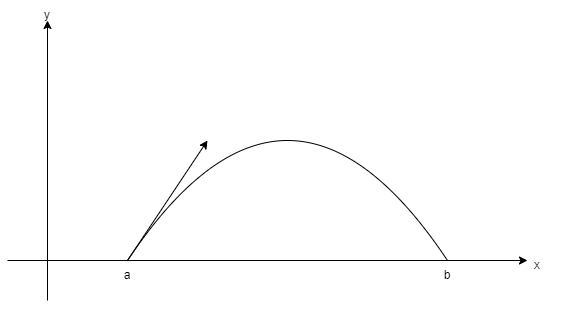
\includegraphics[scale=0.8]{parabola.png}
    \end{figure}

    Seeing the y-axis as the tag for height from the ground, and seeing x-axis as the tag for horizontal distance, we obtain a trajectory for a throwing motion starting from $x=a$ to $x=b$ in the direction indicated by an arrow drawn on the figure. Recall some memory of speed and distance, we have \begin{align*}
        x-a=v_x t
    \end{align*}where $v_x$ indicates the horizontal speed. This modelling satisfies the condition for when $t=0$, $x=a$, and that $v_x$ is constant. We now have $t$ to be the tag for time and we know that the whole motion shares the same time tag, which means for vertical component (i.e. the height) also undergoes the same time parameter $t$, so that \begin{align*}
        v_y=u_y-gt
    \end{align*}
    is a suitable modelling for the vertical component in which is meaning the vertical velocity is decreasing consistently with respect to the gravity. By the understanding from physicists that \begin{align*}
        y=\frac{u_y+v_y}{2}t
    \end{align*} we have the equation \begin{align*}
        y=u_y t-\frac{1}{2}gt^2
    \end{align*} and by simple substitution of $t=\frac{x-a}{v_x}$ into the equation for $y$ we have an equation for parabola in the form of \begin{align*}
        y=ax^2+bx+c
    \end{align*}

    To investigate the properties of a quadratic curve we introduce the \textbf{method of completing square}:\begin{align*}
        ax^2+bx+c&=a(x^2+\frac{b}{a}x)+c\\
        &=a(x^2+2\frac{b}{2a}x+\frac{b^2}{4a^2}-\frac{b^2}{4a^2})+c\\
        &=a(x+\frac{b}{2a})^2-\frac{b^2-4ac}{4a}\\
        &=a(x+\frac{b}{2a})^2+\frac{4ac-b^2}{4a}
    \end{align*}

    One observation is that when $x+\dfrac{b}{2a}$ attains 0, the polynomial attains its extremum value (maximum or minimum), because for $(x+\frac{b}{2a})^2$ its minimum value is 0, and the polynomial in this form can be controlled by $x+\frac{b}{2a}$. The above form is called the \textbf{vertex form}. Using the vertex form, we can now conclude: \begin{itemize}
        \item The \textbf{vertex} is at $(-\dfrac{b}{2a},\dfrac{4ac-b^2}{4a})$.
        \item The \textbf{axis of symmetry} is $x=-\dfrac{b}{2a}$.
        \item The \textbf{extremum value} is $\dfrac{4ac-b^2}{4a}$.
    \end{itemize}

    We may also notice that when the graph has minimum point, it should be opening upward:

    \begin{figure}[H]
        \centering
        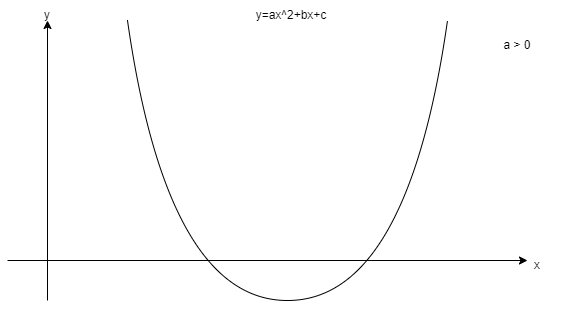
\includegraphics[scale=0.6]{open_upward.png}
    \end{figure}

    and when the graph has maximum point, it should be opening downward:

    \begin{figure}[H]
        \centering
        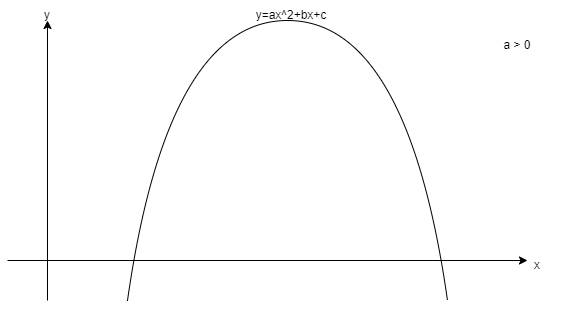
\includegraphics[scale=0.6]{open_downward.png}
    \end{figure}

    \begin{example}
        Using the method of completing square, determine the direction of opening, and find the vertex, axis of symmetry and the minimum value for the graph of $y=2x^2+3x+4$.
    \end{example}

    \textit{ Sol.}\begin{align*}
        2x^2+3x+4&=2(x^2+\frac{3}{2}x)+4\\
        &=2(x^2+2\frac{3}{4}x+\frac{9}{16}-\frac{9}{16})+4\\
        &=2(x+\frac{3}{4})^2+\frac{23}{8}
    \end{align*}
    So, the graph is opening upward, has vertex at $(-\dfrac{3}{4},\dfrac{23}{8})$, axis of symmetry $x=-\dfrac{3}{4}$ and minimum value $\dfrac{23}{8}$.

    \begin{example}
        Find the vertex, axis of symmetry and the extremum value for the graph of $y=kx^2+4x+6$ in terms of $k$.
    \end{example}

    \textit{ Sol.}
    By the formula deduced earlier, the graph has vertex at $(-\dfrac{2}{k},\dfrac{4k-4}{k})$, axis of symmetry $x=-\dfrac{2}{k}$ and extrmum value $\dfrac{4k-4}{k}$.

    \subsection*{Exercise}
    \begin{enumerate}
        \item Using the method of completing square, determine the direction of opening, and find the vertex, axis of symmetry and the minimum value for the following graphs.\begin{align*}
            &a)\ y=2x^2+12x+16&&b)\ y=3x^2+27x+54&&c)\ y=5x^2+35x+30\\
            &d)\ y=7x^2-42x+56&&e)\ y=-11x^2+99x-198&&f)\ y=-3x^2+21x-18
        \end{align*}
        \item Find the vertex, axis of symmetry and the extremum value for the following graphs in terms of $k$.\begin{align*}
            &a)\ y=kx^2-2x+9&&b)\ y=82x^2+kx+79&&c)\ y=-24x^2-70x+4k\\
            &d)\ y=-kx^2+36x-k&&e)\ y=8kx^2+3kx-51&&f)\ y=2kx^2+(3k-6)x-4k-8
        \end{align*}
    \end{enumerate}

    \pagebreak

    \subsection*{Challenging questions}
    \begin{enumerate}
        \item Solve $8x^2+2x+3=2x^2-4$. You may represent your answer in surds and the form of complex number if needed.
        \item Solve the equation $\dfrac{x-3}{2x-3}=\dfrac{7x+3}{2x-5}$. You may represent your answer in surds and the form of complex number if needed.
        \item If $x^2-2ax+a^2=0$, find the value of $\dfrac{x}{a}$.
        \item $\dfrac{x^{2002}+4x^{2001}}{4x^{2000}}=2449.25$.
        \item Find the value of $\sqrt{6+\sqrt{6+\sqrt{6+\sqrt{6+\cdots}}}}$.
        \item If $\alpha,\beta$ are roots of the equation $x^2-8x+11=0$, find the value of $\alpha^3+\alpha^2+\alpha+\beta^3+\beta^2+\beta$.
        \item If $\alpha,\beta$ are real roots to the equation in $x$: $x^2-5x+a^2-2a+1=0$, find the value of $a$ such that $\alpha\beta$ is of minimal value.
        \item Find the value of $\alpha^2+\beta^2+\gamma^2$ where $\alpha,\beta,\gamma$ are the roots of the equation $3x^3-2x^2+5x-7=0$.
        \item Find the value(s) of the positive real number $a$ such that the graph of $$y=(a^2+1)x^2-2ax+10$$ has minimum value $\dfrac{451}{50}$ for $0<x<\dfrac{1}{2}$.
    \end{enumerate}
\end{document}